\documentclass[11pt, letterpaper]{article}

% Fonts and Encoding
\usepackage[utf8]{inputenc}
\usepackage[T1]{fontenc}
\usepackage{lmodern}

% Math and Symbols
\usepackage{amsmath, amssymb, amsthm, amsfonts, mathrsfs, mathtools}

% Layout and Geometry
\usepackage{geometry}
\geometry{letterpaper, margin=1in}
\setlength{\parindent}{0pt}
\setlength{\parskip}{0.6em}

% Formatting and Graphics
\usepackage{graphicx, xcolor, enumitem, booktabs, array, tabularx}

% TikZ for Illustrations
\usepackage{tikz}
\usetikzlibrary{arrows.meta, positioning, shapes.geometric, calc, backgrounds, matrix}

% Clickable Links and TOC
\usepackage{hyperref}
\hypersetup{
    colorlinks=true,
    linkcolor=blue,
    filecolor=magenta,      
    urlcolor=cyan,
    pdftitle={Advanced Mathematics Topic: Applications to Markov Chains},
}

% Theorem Environments
\newtheorem{theorem}{Theorem}[section]
\newtheorem{lemma}[theorem]{Lemma}
\newtheorem{proposition}[theorem]{Proposition}
\newtheorem{corollary}[theorem]{Corollary}
\theoremstyle{definition}
\newtheorem{definition}{Definition}[section]
\newtheorem{axiom}{Axiom}[section]
\newtheorem{example}{Example}[section]
\theoremstyle{remark}
\newtheorem{remark}{Remark}[section]

% Custom Commands (Enforced standard notation)
\newcommand{\R}{\mathbb{R}}
\newcommand{\N}{\mathbb{N}}
\newcommand{\Z}{\mathbb{Z}}
\newcommand{\Q}{\mathbb{Q}}
\newcommand{\E}{\mathbb{E}}
\newcommand{\Prob}{\mathbb{P}}
\newcommand{\F}{\mathcal{F}}

\begin{document}

\title{\textbf{Applications to Markov Chains}\\ \Large Comprehensive Study Guide and Solutions}
\author{Tashfeen Omran}
\date{\today}
\maketitle

\tableofcontents
\newpage

\section{Part 1: Comprehensive Introduction, Context, and Prerequisites}

\subsection{Core Concepts}
A \textbf{Markov chain} is a mathematical system that experiences transitions from one state to another according to certain probabilistic rules. The defining characteristic of a Markov chain is that no matter how the system arrived at its current state, the possible future states are fixed. In other words, the probability of transitioning to any particular state depends solely on the current state and time elapsed, not on the sequence of state that preceded it. This is known as the \textit{Markov property} or \textit{memorylessness}.

In linear algebra, we model these systems using vectors and matrices:
\begin{itemize}
    \item \textbf{Probability Vector:} A vector with non-negative entries that add up to $1$. It represents a probability distribution across various states.
    \item \textbf{Stochastic Matrix ($P$):} A square matrix whose columns are probability vectors. The entry $P_{ij}$ represents the probability of transitioning \textit{to} state $i$ \textit{from} state $j$.
    \item \textbf{State Vector ($x_k$):} A probability vector representing the state of the system at time step $k$. The evolution of the system is given by the first-order difference equation:
    \[ x_{k+1} = P x_k \quad \text{for} \quad k = 0, 1, 2, \dots \]
    \item \textbf{Steady-State Vector ($q$):} A probability vector $q$ such that $Pq = q$. It represents an equilibrium distribution where the probabilities no longer change from one step to the next.
\end{itemize}

\subsection{Intuition and Derivation}
Imagine a population moving between a City and its Suburbs. If $5\%$ of city dwellers move to the suburbs each year, and $3\%$ of suburbanites move to the city, the total population is conserved, but its distribution changes. The matrix $P$ captures these transition rates. Multiplying $P$ by the current distribution $x_k$ computes the new distribution $x_{k+1}$ by taking a linear combination of the transition probabilities weighted by the current population in each state. 

Finding the long-term behavior requires finding a vector that remains unchanged after being multiplied by $P$. Mathematically, this is the definition of an eigenvector corresponding to the eigenvalue $\lambda = 1$. Because the columns of a stochastic matrix sum to $1$, it is guaranteed (by Theorem 10) that $\lambda = 1$ is always an eigenvalue.

\subsection{Historical Context and Motivation}
The theory of Markov chains was developed by the Russian mathematician Andrey Markov in 1906. Prior to his work, probability theory largely focused on \textit{independent} events (like coin flips). Markov wanted to prove that the Law of Large Numbers could apply to \textit{dependent} events as well. He famously applied his theory to analyze the sequence of vowels and consonants in Alexander Pushkin's novel \textit{Eugene Onegin}, birthing the mathematical study of stochastic processes which now underpins modern physics, genetics, and artificial intelligence.

\subsection{Key Formulas}
\begin{enumerate}
    \item \textbf{State Evolution:} $x_k = P^k x_0$
    \item \textbf{Steady-State Equation:} $Pq = q \implies (P - I)q = 0$
    \item \textbf{Probability Constraint:} $\sum_{i=1}^n q_i = 1$
\end{enumerate}

\subsection{Prerequisites}
To master this topic, you must be proficient in:
\begin{itemize}
    \item \textbf{Matrix Multiplication:} Understanding how to compute $Px$.
    \item \textbf{Null Spaces and Row Reduction:} Solving homogeneous systems $(P - I)x = 0$ using augmented matrices and row operations.
    \item \textbf{Eigenvalues and Eigenvectors:} Recognizing that finding a steady-state vector is equivalent to finding an eigenvector for $\lambda = 1$.
\end{itemize}

\newpage
\section{Part 2: Detailed Homework Solutions}
\textit{Note: In accordance with strategic learning protocols, a representative sample of problems covering every distinct archetype has been selected from the text to maximize conceptual coverage without redundant repetition.}

\subsection{Type 1: Modeling and Setup}

\textbf{Problem 1:} A small remote village receives radio broadcasts from two radio stations, a news station and a music station. Of the listeners who are tuned to the news station, $70\%$ will remain listening to the news after the station break, while $30\%$ will switch to the music station. Of the listeners who are tuned to the music station, $60\%$ will switch to the news station, while $40\%$ will remain listening to the music. Suppose everyone is listening to the news at 8:15 A.M.
\begin{enumerate}[label=\alph*.]
    \item Give the stochastic matrix that describes how the radio listeners tend to change stations.
    \item Give the initial state vector.
    \item What percentage of the listeners will be listening to the music station at 9:25 A.M. (after the station breaks at 8:30 and 9:00 A.M.)?
\end{enumerate}

\textbf{Solution:}
\textbf{Part a:} Let State 1 be the News station and State 2 be the Music station. The columns represent the \textit{current} state (From) and the rows represent the \textit{next} state (To).
\[ P = \begin{bmatrix} 0.7 & 0.6 \\ 0.3 & 0.4 \end{bmatrix} \quad \begin{array}{l} \text{News} \\ \text{Music} \end{array} \]

\textbf{Part b:} At 8:15 A.M., $100\%$ of the listeners are on the news station.
\[ x_0 = \begin{bmatrix} 1 \\ 0 \end{bmatrix} \]

\textbf{Part c:} We need to find the state after two station breaks (8:30 A.M. is $k=1$, 9:00 A.M. is $k=2$). The time 9:25 A.M. falls after the second break but before the third.
First, compute $x_1$:
\[ x_1 = P x_0 = \begin{bmatrix} 0.7 & 0.6 \\ 0.3 & 0.4 \end{bmatrix} \begin{bmatrix} 1 \\ 0 \end{bmatrix} = \begin{bmatrix} 0.7 \\ 0.3 \end{bmatrix} \]
Next, compute $x_2$:
\[ x_2 = P x_1 = \begin{bmatrix} 0.7 & 0.6 \\ 0.3 & 0.4 \end{bmatrix} \begin{bmatrix} 0.7 \\ 0.3 \end{bmatrix} = \begin{bmatrix} (0.7)(0.7) + (0.6)(0.3) \\ (0.3)(0.7) + (0.4)(0.3) \end{bmatrix} = \begin{bmatrix} 0.49 + 0.18 \\ 0.21 + 0.12 \end{bmatrix} = \begin{bmatrix} 0.67 \\ 0.33 \end{bmatrix} \]
The second entry represents the music station. Therefore, \textbf{$33\%$} of the listeners will be listening to the music station at 9:25 A.M.

\vspace{1em}
\textbf{Problem 2:} A laboratory animal may eat any one of three foods each day. If the animal chooses one food on one trial, it will choose the same food on the next trial with a probability of $50\%$, and it will choose the other foods on the next trial with equal probabilities of $25\%$.
\begin{enumerate}[label=\alph*.]
    \item What is the stochastic matrix for this situation?
    \item If the animal chooses food \#1 on an initial trial, what is the probability that it will choose food \#2 on the second trial after the initial trial?
\end{enumerate}

\textbf{Solution:}
\textbf{Part a:} The matrix $P$ will be $3 \times 3$. The diagonal entries (staying with the same food) are $0.50$. The off-diagonal entries (switching to another food) are $0.25$.
\[ P = \begin{bmatrix} 0.50 & 0.25 & 0.25 \\ 0.25 & 0.50 & 0.25 \\ 0.25 & 0.25 & 0.50 \end{bmatrix} \]

\textbf{Part b:} The initial state is $x_0 = \begin{bmatrix} 1 \\ 0 \\ 0 \end{bmatrix}$. We want the probability of food \#2 at $k=2$ (the second trial after the initial).
\[ x_1 = P x_0 = \begin{bmatrix} 0.50 \\ 0.25 \\ 0.25 \end{bmatrix} \]
\[ x_2 = P x_1 = \begin{bmatrix} 0.50 & 0.25 & 0.25 \\ 0.25 & 0.50 & 0.25 \\ 0.25 & 0.25 & 0.50 \end{bmatrix} \begin{bmatrix} 0.50 \\ 0.25 \\ 0.25 \end{bmatrix} = \begin{bmatrix} (0.5)(0.5) + (0.25)(0.25) + (0.25)(0.25) \\ (0.25)(0.5) + (0.5)(0.25) + (0.25)(0.25) \\ (0.25)(0.5) + (0.25)(0.25) + (0.5)(0.25) \end{bmatrix} \]
Calculating the second entry (Food \#2):
\[ (0.25)(0.50) + (0.50)(0.25) + (0.25)(0.25) = 0.125 + 0.125 + 0.0625 = 0.3125 \]
The probability is \textbf{$31.25\%$}.

\subsection{Type 2: Finding Steady-State Vectors}

\textbf{Problem 5:} Find the steady-state vector for $P = \begin{bmatrix} 0.1 & 0.6 \\ 0.9 & 0.4 \end{bmatrix}$.

\textbf{Solution:}
We must solve $(P - I)q = 0$.
\[ P - I = \begin{bmatrix} 0.1 - 1 & 0.6 \\ 0.9 & 0.4 - 1 \end{bmatrix} = \begin{bmatrix} -0.9 & 0.6 \\ 0.9 & -0.6 \end{bmatrix} \]
Set up the augmented matrix and row reduce:
\[ \begin{bmatrix} -0.9 & 0.6 & 0 \\ 0.9 & -0.6 & 0 \end{bmatrix} \xrightarrow{R_2 + R_1 \to R_2} \begin{bmatrix} -0.9 & 0.6 & 0 \\ 0 & 0 & 0 \end{bmatrix} \xrightarrow{-\frac{10}{9}R_1 \to R_1} \begin{bmatrix} 1 & -2/3 & 0 \\ 0 & 0 & 0 \end{bmatrix} \]
This gives the equation $x_1 - \frac{2}{3}x_2 = 0$, so $x_1 = \frac{2}{3}x_2$. Let $x_2 = 3$, then $x_1 = 2$. A basis vector for the null space is $v = \begin{bmatrix} 2 \\ 3 \end{bmatrix}$.
To make it a probability vector, divide by the sum of its entries ($2+3=5$):
\[ q = \begin{bmatrix} 2/5 \\ 3/5 \end{bmatrix} = \begin{bmatrix} 0.4 \\ 0.6 \end{bmatrix} \]

\vspace{1em}
\textbf{Problem 7:} Find the steady-state vector for $P = \begin{bmatrix} 0.7 & 0.1 & 0.1 \\ 0.2 & 0.8 & 0.2 \\ 0.1 & 0.1 & 0.7 \end{bmatrix}$.

\textbf{Solution:}
Solve $(P - I)q = 0$.
\[ P - I = \begin{bmatrix} -0.3 & 0.1 & 0.1 \\ 0.2 & -0.2 & 0.2 \\ 0.1 & 0.1 & -0.3 \end{bmatrix} \]
Multiply by $10$ to clear decimals:
\[ \begin{bmatrix} -3 & 1 & 1 \\ 2 & -2 & 2 \\ 1 & 1 & -3 \end{bmatrix} \]
Row reduce the augmented matrix:
\[ \begin{bmatrix} -3 & 1 & 1 & 0 \\ 2 & -2 & 2 & 0 \\ 1 & 1 & -3 & 0 \end{bmatrix} \xrightarrow{R_1 \leftrightarrow R_3} \begin{bmatrix} 1 & 1 & -3 & 0 \\ 2 & -2 & 2 & 0 \\ -3 & 1 & 1 & 0 \end{bmatrix} \]
\[ \xrightarrow{R_2 - 2R_1 \to R_2, \ R_3 + 3R_1 \to R_3} \begin{bmatrix} 1 & 1 & -3 & 0 \\ 0 & -4 & 8 & 0 \\ 0 & 4 & -8 & 0 \end{bmatrix} \]
\[ \xrightarrow{R_3 + R_2 \to R_3, \ -\frac{1}{4}R_2 \to R_2} \begin{bmatrix} 1 & 1 & -3 & 0 \\ 0 & 1 & -2 & 0 \\ 0 & 0 & 0 & 0 \end{bmatrix} \]
\[ \xrightarrow{R_1 - R_2 \to R_1} \begin{bmatrix} 1 & 0 & -1 & 0 \\ 0 & 1 & -2 & 0 \\ 0 & 0 & 0 & 0 \end{bmatrix} \]
This yields $x_1 = x_3$ and $x_2 = 2x_3$. Let $x_3 = 1$, giving the basis vector $v = \begin{bmatrix} 1 \\ 2 \\ 1 \end{bmatrix}$.
Sum of entries $= 1 + 2 + 1 = 4$.
\[ q = \begin{bmatrix} 1/4 \\ 2/4 \\ 1/4 \end{bmatrix} = \begin{bmatrix} 0.25 \\ 0.50 \\ 0.25 \end{bmatrix} \]

\subsection{Type 3: Regular Stochastic Matrices}

\textbf{Problem 9:} Determine if $P = \begin{bmatrix} 0.7 & 0 \\ 0.3 & 1 \end{bmatrix}$ is a regular stochastic matrix.

\textbf{Solution:}
A stochastic matrix is regular if some matrix power $P^k$ contains \textit{only strictly positive} entries ($>0$).
Let's compute $P^2$:
\[ P^2 = \begin{bmatrix} 0.7 & 0 \\ 0.3 & 1 \end{bmatrix} \begin{bmatrix} 0.7 & 0 \\ 0.3 & 1 \end{bmatrix} = \begin{bmatrix} 0.49 & 0 \\ 0.21 + 0.3 & 1 \end{bmatrix} = \begin{bmatrix} 0.49 & 0 \\ 0.51 & 1 \end{bmatrix} \]
Notice that the top-right entry remains $0$. In fact, for any $k$, the top-right entry of $P^k$ will be $0$ because state 2 is an \textit{absorbing state} (once you enter state 2, you never leave, hence the $1$ in the bottom right and $0$ above it). Therefore, $P$ is \textbf{not regular}.

\vspace{1em}
\textbf{Problem 10:} Determine if $P = \begin{bmatrix} 0 & 0.7 \\ 1 & 0.3 \end{bmatrix}$ is a regular stochastic matrix.

\textbf{Solution:}
Check $P^2$:
\[ P^2 = \begin{bmatrix} 0 & 0.7 \\ 1 & 0.3 \end{bmatrix} \begin{bmatrix} 0 & 0.7 \\ 1 & 0.3 \end{bmatrix} = \begin{bmatrix} 0(0) + 0.7(1) & 0(0.7) + 0.7(0.3) \\ 1(0) + 0.3(1) & 1(0.7) + 0.3(0.3) \end{bmatrix} = \begin{bmatrix} 0.7 & 0.21 \\ 0.3 & 0.79 \end{bmatrix} \]
Since all entries in $P^2$ are strictly greater than $0$, $P$ is \textbf{regular}.

\subsection{Type 4: True/False Conceptual Analysis}

\textbf{Problem 15:} (T/F) The steady state vector is an eigenvector of $P$.
\textbf{Solution:} \textbf{True}. By definition, a steady-state vector $q$ satisfies $Pq = q$, which can be written as $Pq = 1 \cdot q$. This means $q$ is an eigenvector of $P$ corresponding to the eigenvalue $\lambda = 1$.

\textbf{Problem 16:} (T/F) Every eigenvector of $P$ is a steady state vector.
\textbf{Solution:} \textbf{False}. An eigenvector of $P$ might correspond to an eigenvalue other than $1$. Furthermore, even if it corresponds to $\lambda = 1$, an eigenvector is not a steady-state vector unless its entries are non-negative and sum to $1$ (it must be a probability vector).

\textbf{Problem 17:} (T/F) The all ones vector is an eigenvector of $P^T$.
\textbf{Solution:} \textbf{True}. Let $\mathbf{1}$ be the vector of all ones. Because $P$ is a stochastic matrix, the sum of the entries in each column is $1$. Therefore, the sum of the entries in each \textit{row} of $P^T$ is $1$. Multiplying $P^T \mathbf{1}$ sums the rows of $P^T$, resulting in a vector of all ones. Thus, $P^T \mathbf{1} = 1 \cdot \mathbf{1}$.

\subsection{Type 5: Verifying Steady-State Vectors}

\textbf{Problem 21:} Is $q = \begin{bmatrix} 0.6 \\ 0.8 \end{bmatrix}$ a steady state vector for $A = \begin{bmatrix} 0.2 & 0.6 \\ 0.8 & 0.4 \end{bmatrix}$? Justify your answer.

\textbf{Solution:}
\textbf{No.} A steady-state vector must be a probability vector. The sum of the entries of $q$ is $0.6 + 0.8 = 1.4 \neq 1$. Even though $Aq = q$ happens to be true here, $q$ fails the definition of a state vector.

\subsection{Type 6: Advanced Theoretical Proofs}

\textbf{Problem 28:} Show that every $2 \times 2$ stochastic matrix has at least one steady-state vector. Any such matrix can be written in the form $P = \begin{bmatrix} 1-\alpha & \beta \\ \alpha & 1-\beta \end{bmatrix}$, where $\alpha$ and $\beta$ are constants between $0$ and $1$.

\textbf{Solution:}
To find the steady-state vector, we solve $(P - I)x = 0$.
\[ P - I = \begin{bmatrix} 1-\alpha - 1 & \beta \\ \alpha & 1-\beta - 1 \end{bmatrix} = \begin{bmatrix} -\alpha & \beta \\ \alpha & -\beta \end{bmatrix} \]
Row reducing this matrix:
\[ \begin{bmatrix} -\alpha & \beta & 0 \\ \alpha & -\beta & 0 \end{bmatrix} \xrightarrow{R_2 + R_1 \to R_2} \begin{bmatrix} -\alpha & \beta & 0 \\ 0 & 0 & 0 \end{bmatrix} \]
This gives the equation $-\alpha x_1 + \beta x_2 = 0$, or $\alpha x_1 = \beta x_2$.
A natural choice for a basis vector of the null space is $v = \begin{bmatrix} \beta \\ \alpha \end{bmatrix}$.
To make this a probability vector, we divide by the sum of its entries ($\alpha + \beta$):
\[ q = \begin{bmatrix} \frac{\beta}{\alpha + \beta} \\ \frac{\alpha}{\alpha + \beta} \end{bmatrix} \]
As long as $\alpha$ and $\beta$ are not both zero, this unique steady-state vector exists. If $\alpha = \beta = 0$, then $P = I$, and any probability vector is a steady-state vector.

\newpage
\section{Part 3: In-Depth Analysis of Problems and Techniques}

\subsection{A) Problem Types and General Approach}
\begin{itemize}
    \item \textbf{Modeling/Setup Problems (Ex 1, 2):} 
    \textit{Strategy:} Carefully read the prompt to identify the states. The phrase "Of those in state A, X\% go to state B" means the column for A will have X\% in the row for B. Always verify that every column sums to exactly $1$. Use $x_k = P^k x_0$ to find future states.
    \item \textbf{Steady-State Calculation Problems (Ex 5, 7):}
    \textit{Strategy:} Set up the homogeneous system $(P - I)x = 0$. Row reduce to find the parametric vector form of the null space. Choose a convenient basis vector (usually by picking a free variable that clears fractions), and then \textit{normalize} it by dividing by the sum of its components.
    \item \textbf{Regularity Checks (Ex 9, 10):}
    \textit{Strategy:} Check if $P$ has any zero entries. If it doesn't, it's regular ($k=1$). If it does, compute $P^2, P^3$, etc. If you find a power where all entries are strictly positive, it is regular. If a zero persists in the same location (often due to an absorbing state), it is not regular.
\end{itemize}

\subsection{B) Key Algebraic and Calculus Manipulations}
\begin{itemize}
    \item \textbf{Clearing Decimals Before Row Reduction:} In Problem 7, the matrix $P-I$ contained decimals like $-0.3$ and $0.1$. Multiplying the entire augmented matrix by $10$ before row reducing prevents floating-point arithmetic errors and makes finding the exact fractional basis vector much easier.
    \item \textbf{The Normalization Trick:} When solving $(P-I)x = 0$, the resulting vector is just a basis for the eigenspace. To convert it to a Markov steady-state vector, you must apply the $L_1$ norm constraint: $q = \frac{v}{\sum v_i}$.
    \item \textbf{The $2 \times 2$ Shortcut:} As proven in Problem 28, for any $2 \times 2$ matrix $P = \begin{bmatrix} 1-\alpha & \beta \\ \alpha & 1-\beta \end{bmatrix}$, the steady state is always $q = \frac{1}{\alpha+\beta}\begin{bmatrix} \beta \\ \alpha \end{bmatrix}$. This allows you to bypass row reduction entirely for $2 \times 2$ matrices.
\end{itemize}

\newpage
\section{Part 4: "Cheatsheet" and Tips for Success}

\subsection{Summary of Important Formulas}
\renewcommand{\arraystretch}{1.5}
\begin{tabularx}{\textwidth}{>{\hsize=0.3\hsize\bfseries}X >{\hsize=0.7\hsize}X}
\toprule
Concept & Formula / Definition \\
\midrule
State Evolution & $x_k = P^k x_0$ \\
Steady-State Condition & $Pq = q \iff (P - I)q = 0$ \\
Probability Constraint & $\sum_{i=1}^n q_i = 1$ and $q_i \geq 0$ \\
$2 \times 2$ Shortcut & If $P = \begin{bmatrix} 1-\alpha & \beta \\ \alpha & 1-\beta \end{bmatrix}$, then $q = \begin{bmatrix} \frac{\beta}{\alpha+\beta} \\[4pt] \frac{\alpha}{\alpha+\beta} \end{bmatrix}$ \\
\bottomrule
\end{tabularx}

\subsection{Tricks and Shortcuts}
\begin{itemize}
    \item \textbf{The Column Sum Check:} After computing $P-I$, immediately check the columns. The sum of the entries in \textit{every} column of $P-I$ must be exactly $0$. If they do not sum to $0$, you made an arithmetic error in your setup.
    \item \textbf{Free Variable Selection:} When finding the null space basis, if your equations are $x_1 = \frac{3}{4}x_3$ and $x_2 = \frac{1}{2}x_3$, choose $x_3 = 4$ (the common denominator) to get a basis vector of integers: $\begin{bmatrix} 3 \\ 2 \\ 4 \end{bmatrix}$. This makes the final normalization step much cleaner.
\end{itemize}

\subsection{Common Pitfalls to Avoid}
\begin{itemize}
    \item \textbf{Rows vs. Columns:} The most common mistake is setting up $P$ such that the \textit{rows} sum to 1. In standard Markov chain notation (right-multiplying column vectors), the \textbf{columns} must sum to 1.
    \item \textbf{Forgetting to Normalize:} Finding the eigenvector $\begin{bmatrix} 2 \\ 3 \end{bmatrix}$ and stopping. You will lose points. You must divide by $5$ to get $\begin{bmatrix} 0.4 \\ 0.6 \end{bmatrix}$.
    \item \textbf{Misinterpreting "Regular":} A matrix with zeros can still be regular! You must check $P^2, P^3$, etc. Do not assume a single zero in $P$ means it is not regular.
\end{itemize}

\vspace{2em}
\begin{center}
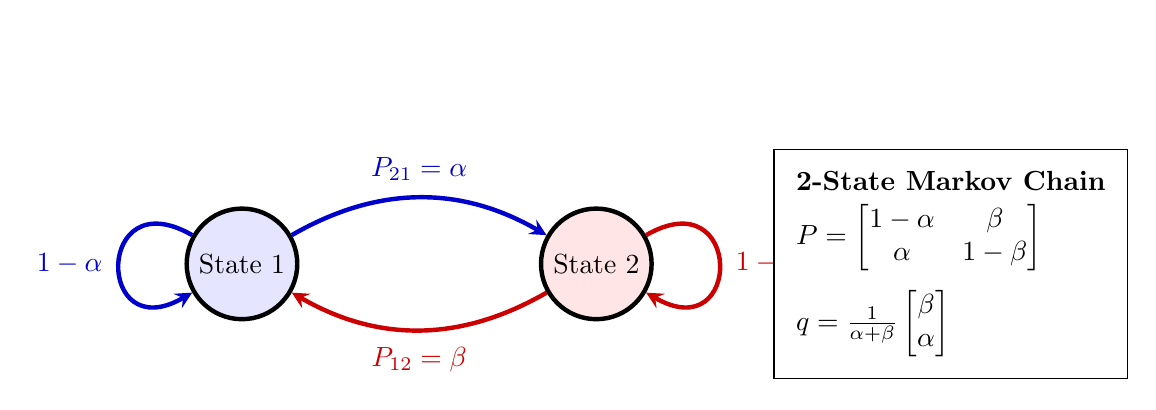
\begin{tikzpicture}[scale=1.5]
    % Background fill to ensure safe rendering
    \fill[white] (-1,-1) rectangle (4,2);
    
    % Nodes
    \node[circle, draw, ultra thick, fill=blue!10, minimum size=1.2cm] (A) at (0,0) {State 1};
    \node[circle, draw, ultra thick, fill=red!10, minimum size=1.2cm] (B) at (3,0) {State 2};
    
    % Edges
    \draw[->, >=stealth, ultra thick, blue!80!black] (A) to[bend left=30] node[above=2pt] {$P_{21} = \alpha$} (B);
    \draw[->, >=stealth, ultra thick, red!80!black] (B) to[bend left=30] node[below=2pt] {$P_{12} = \beta$} (A);
    
    % Self loops
    \draw[->, >=stealth, ultra thick, blue!80!black] (A) to[loop left, out=150, in=210, looseness=5] node[left=2pt] {$1-\alpha$} (A);
    \draw[->, >=stealth, ultra thick, red!80!black] (B) to[loop right, out=30, in=-30, looseness=5] node[right=2pt] {$1-\beta$} (B);
    
    % Legend Node
    \node[align=left, draw, fill=white, inner sep=8pt, anchor=west] at (4.5, 0) {
        \textbf{2-State Markov Chain}\\[4pt]
        $P = \begin{bmatrix} 1-\alpha & \beta \\ \alpha & 1-\beta \end{bmatrix}$\\[6pt]
        $q = \frac{1}{\alpha+\beta} \begin{bmatrix} \beta \\ \alpha \end{bmatrix}$
    };
\end{tikzpicture}
\end{center}

\newpage
\section{Part 5: Conceptual Synthesis and The "Big Picture"}

\subsection{A) Thematic Connections}
The core theme of this topic is \textbf{long-term equilibrium in dynamic systems}. We are using static linear algebra tools (eigenvalues and null spaces) to understand a system that is constantly in motion. This mirrors the concept of \textit{limits} in calculus. Just as $\lim_{x \to \infty} f(x)$ tells us the horizontal asymptote of a function, $\lim_{k \to \infty} P^k x_0 = q$ tells us the "asymptote" of a probability distribution. The system reaches a state of dynamic equilibrium where the macroscopic distribution remains constant even though microscopic individual transitions are still occurring.

\subsection{B) Forward and Backward Links}
\textbf{Backward Links:} This topic is the ultimate culmination of Chapter 5 (Eigenvalues and Eigenvectors). It provides a concrete, physical interpretation of what an eigenvector actually is: a state that is invariant under a transformation. It also relies heavily on Chapter 1 (solving homogeneous systems $Ax = 0$).

\textbf{Forward Links:} Understanding discrete Markov chains is the absolute bedrock for studying \textit{Stochastic Processes} and \textit{Continuous-Time Markov Chains}. In later courses, the discrete time steps ($k=1, 2, \dots$) become a continuous time variable $t$, and the transition matrix $P$ is replaced by a transition rate matrix (Generator matrix $Q$), leading to systems of differential equations (Kolmogorov equations).

\section{Part 6: Abstract Real-World Modeling (AI, ML, \& Quant Finance)}

\subsection{A) Concrete Scenarios}
\begin{enumerate}
    \item \textbf{Generative AI \& Natural Language Processing:} Large Language Models (LLMs) are fundamentally highly advanced, continuous-space extensions of Markov chains. A basic $N$-gram model predicts the next word based strictly on the previous $N$ words (the Markov property). The transition matrix contains the probabilities of word $j$ following word $i$ based on training corpus frequencies.
    \item \textbf{Algorithmic Trading (Regime Switching Models):} Financial markets shift between distinct "regimes" (e.g., High Volatility/Bear Market vs. Low Volatility/Bull Market). Quants use Hidden Markov Models (HMMs) where the underlying market regime is a Markov chain, and the observed asset returns are drawn from a probability distribution dependent on the current hidden state.
    \item \textbf{Quantitative Finance (Credit Rating Migration):} Corporate bonds are rated by agencies (AAA, AA, A, BBB, Default). The probability that a bond gets upgraded or downgraded over a year is modeled as a Markov chain. Pricing credit derivatives (like Credit Default Swaps) requires calculating the exact probability that a bond will hit the "Default" absorbing state before maturity.
\end{enumerate}

\subsection{B) Model Problem Setup: Credit Rating Migration}
Let us rigorously formulate the Credit Rating Migration model. Define a finite state space $\mathcal{S} = \{1, 2, 3, 4\}$, representing ratings $\{\text{AAA}, \text{BBB}, \text{CCC}, \text{Default}\}$. State 4 (Default) is an \textit{absorbing state}.
Let $(\Omega, \F, \Prob)$ be a probability space, and let $X_t : \Omega \to \mathcal{S}$ be a stochastic process representing the rating of a bond at year $t \in \N$. The evolution is governed by the transition matrix $P \in \R^{4 \times 4}$:
\[ P = \begin{bmatrix} 
0.90 & 0.05 & 0.00 & 0.00 \\
0.08 & 0.85 & 0.10 & 0.00 \\
0.02 & 0.08 & 0.70 & 0.00 \\
0.00 & 0.02 & 0.20 & 1.00 
\end{bmatrix} \]
Notice that $P_{44} = 1$, ensuring that once $X_t = 4$, $X_{t+k} = 4$ almost surely for all $k > 0$.
A quantitative researcher needs to price a 5-year zero-coupon bond currently rated BBB (State 2). The payout is $\$100$ if it does not default, and $\$0$ if it defaults. The expected payoff under the physical measure is:
\[ \E[\text{Payoff}] = 100 \times \Prob(X_5 \neq 4 \mid X_0 = 2) \]
To compute this, we calculate the state vector at $t=5$: $x_5 = P^5 e_2$, where $e_2 = \begin{bmatrix} 0 & 1 & 0 & 0 \end{bmatrix}^T$. The probability of survival is $1 - (x_5)_4$. This discrete Markov framework forms the foundation of the Jarrow-Turnbull model for credit risk.

\newpage
\section{Part 7: Common Variations and Untested Concepts}

\subsection{Missing Concept: Absorbing Markov Chains}
The homework strictly focused on \textit{regular} stochastic matrices, which guarantee a unique steady-state vector where all entries are positive. However, a massive subset of Markov theory deals with \textbf{Absorbing Markov Chains}. 
A state is absorbing if it is impossible to leave (the diagonal entry is $1$). If a chain has absorbing states, we don't look for a standard steady-state vector; instead, we want to know: \textit{How long will it take to get absorbed?} and \textit{Which absorbing state will we end up in?}

\textbf{The Fundamental Matrix ($N$):}
To analyze this, we partition the transition matrix $P$ into transient and absorbing states:
\[ P = \begin{bmatrix} Q & 0 \\ R & I \end{bmatrix} \]
Where $Q$ is the matrix of transitions between transient states. The fundamental matrix is defined as:
\[ N = (I - Q)^{-1} \]
The entry $N_{ij}$ gives the expected number of times the system will visit transient state $i$ given it started in transient state $j$ before eventually being absorbed.

\textbf{Worked Example:}
Consider a student taking a math test. They can be in state 1 (Thinking), state 2 (Guessing), or state 3 (Finished). Finished is an absorbing state.
\[ P = \begin{bmatrix} 0.5 & 0.2 & 0 \\ 0.3 & 0.4 & 0 \\ 0.2 & 0.4 & 1 \end{bmatrix} \quad \begin{array}{l} \text{Thinking} \\ \text{Guessing} \\ \text{Finished} \end{array} \]
The transient matrix $Q$ is the top-left $2 \times 2$ block:
\[ Q = \begin{bmatrix} 0.5 & 0.2 \\ 0.3 & 0.4 \end{bmatrix} \]
We find $N = (I - Q)^{-1}$:
\[ I - Q = \begin{bmatrix} 0.5 & -0.2 \\ -0.3 & 0.6 \end{bmatrix} \]
\[ N = \frac{1}{(0.5)(0.6) - (-0.2)(-0.3)} \begin{bmatrix} 0.6 & 0.2 \\ 0.3 & 0.5 \end{bmatrix} = \frac{1}{0.24} \begin{bmatrix} 0.6 & 0.2 \\ 0.3 & 0.5 \end{bmatrix} = \begin{bmatrix} 2.5 & 0.833 \\ 1.25 & 2.083 \end{bmatrix} \]
If the student starts in the "Thinking" state (column 1), the expected total time steps before finishing is the sum of the first column of $N$: $2.5 + 1.25 = 3.75$ steps.

\newpage
\section{Part 8: Advanced Diagnostic Testing: "Find the Flaw"}

Below are five problems with solutions that contain a subtle, critical flaw. Act as the grader: identify the error, explain why it is wrong in one sentence, and provide the correct solution.

\vspace{1em}
\textbf{Problem 1:} Find the steady-state vector for $P = \begin{bmatrix} 0.8 & 0.5 \\ 0.2 & 0.5 \end{bmatrix}$.
\textit{Flawed Solution:} We solve $(P-I)x = 0$. $P-I = \begin{bmatrix} -0.2 & 0.5 \\ 0.2 & -0.5 \end{bmatrix}$. Row reducing gives $\begin{bmatrix} -0.2 & 0.5 \\ 0 & 0 \end{bmatrix}$. Thus $-0.2x_1 + 0.5x_2 = 0 \implies 2x_1 = 5x_2$. Let $x_2 = 2$, then $x_1 = 5$. The steady state vector is $q = \begin{bmatrix} 5 \\ 2 \end{bmatrix}$.

\textbf{Grader's Correction:}
\textit{Flaw:} The student forgot to normalize the vector so that its entries sum to $1$.
\textit{Correct Solution:} The basis vector is $v = \begin{bmatrix} 5 \\ 2 \end{bmatrix}$. The sum of the entries is $7$. The correct steady-state probability vector is $q = \begin{bmatrix} 5/7 \\ 2/7 \end{bmatrix}$.

\vspace{1em}
\textbf{Problem 2:} A weather model says if it rains today, there is a $60\%$ chance of rain tomorrow and $40\%$ chance of sun. If it is sunny today, there is a $70\%$ chance of sun tomorrow and $30\%$ chance of rain. Set up the stochastic matrix $P$.
\textit{Flawed Solution:} 
\[ P = \begin{bmatrix} 0.6 & 0.4 \\ 0.3 & 0.7 \end{bmatrix} \quad \begin{array}{l} \text{Rain} \\ \text{Sun} \end{array} \]

\textbf{Grader's Correction:}
\textit{Flaw:} The student set up the matrix so that the \textit{rows} sum to 1, but for standard state vectors $x_{k+1} = Px_k$, the \textit{columns} must sum to 1 (representing transitions \textit{from} a specific state).
\textit{Correct Solution:} 
\[ P = \begin{bmatrix} 0.6 & 0.3 \\ 0.4 & 0.7 \end{bmatrix} \]

\vspace{1em}
\textbf{Problem 3:} Determine if $P = \begin{bmatrix} 0.2 & 0.5 & 0 \\ 0.4 & 0.5 & 0.5 \\ 0.4 & 0 & 0.5 \end{bmatrix}$ is regular.
\textit{Flawed Solution:} A matrix is regular if all of its entries are strictly positive. Because $P_{13} = 0$ and $P_{32} = 0$, the matrix contains zeros. Therefore, $P$ is not regular.

\textbf{Grader's Correction:}
\textit{Flaw:} The definition of regular is that \textit{some power} $P^k$ has strictly positive entries, not necessarily $P^1$.
\textit{Correct Solution:} We must check $P^2$. 
\[ P^2 = \begin{bmatrix} 0.2 & 0.5 & 0 \\ 0.4 & 0.5 & 0.5 \\ 0.4 & 0 & 0.5 \end{bmatrix} \begin{bmatrix} 0.2 & 0.5 & 0 \\ 0.4 & 0.5 & 0.5 \\ 0.4 & 0 & 0.5 \end{bmatrix} = \begin{bmatrix} 0.24 & 0.35 & 0.25 \\ 0.48 & 0.45 & 0.50 \\ 0.28 & 0.20 & 0.25 \end{bmatrix} \]
Since all entries in $P^2$ are strictly positive ($>0$), the matrix \textbf{is regular}.

\vspace{1em}
\textbf{Problem 4:} Given $P = \begin{bmatrix} 0.9 & 0.2 \\ 0.1 & 0.8 \end{bmatrix}$ and initial state $x_0 = \begin{bmatrix} 0.5 \\ 0.5 \end{bmatrix}$, find $x_1$.
\textit{Flawed Solution:} $x_1 = P^T x_0 = \begin{bmatrix} 0.9 & 0.1 \\ 0.2 & 0.8 \end{bmatrix} \begin{bmatrix} 0.5 \\ 0.5 \end{bmatrix} = \begin{bmatrix} 0.5 \\ 0.5 \end{bmatrix}$.

\textbf{Grader's Correction:}
\textit{Flaw:} The student multiplied by the transpose $P^T$ instead of the standard transition matrix $P$.
\textit{Correct Solution:} $x_1 = P x_0 = \begin{bmatrix} 0.9 & 0.2 \\ 0.1 & 0.8 \end{bmatrix} \begin{bmatrix} 0.5 \\ 0.5 \end{bmatrix} = \begin{bmatrix} 0.45 + 0.1 \\ 0.05 + 0.4 \end{bmatrix} = \begin{bmatrix} 0.55 \\ 0.45 \end{bmatrix}$.

\vspace{1em}
\textbf{Problem 5:} Verify if $q = \begin{bmatrix} 1.5 \\ -0.5 \end{bmatrix}$ is a steady-state vector for $P = \begin{bmatrix} 0.5 & -1.5 \\ 0.5 & 2.5 \end{bmatrix}$.
\textit{Flawed Solution:} We check if $Pq = q$. 
\[ Pq = \begin{bmatrix} 0.5 & -1.5 \\ 0.5 & 2.5 \end{bmatrix} \begin{bmatrix} 1.5 \\ -0.5 \end{bmatrix} = \begin{bmatrix} 0.75 + 0.75 \\ 0.75 - 1.25 \end{bmatrix} = \begin{bmatrix} 1.5 \\ -0.5 \end{bmatrix} \]
Since $Pq = q$ and the sum of the entries is $1.5 + (-0.5) = 1$, $q$ is a valid steady-state vector.

\textbf{Grader's Correction:}
\textit{Flaw:} A steady-state vector must be a \textit{probability vector}, meaning all entries must be non-negative ($q_i \geq 0$).
\textit{Correct Solution:} Because $q_2 = -0.5 < 0$, $q$ is not a probability vector. Furthermore, $P$ itself is not a valid stochastic matrix because it contains negative entries and entries greater than 1. Therefore, no valid steady-state probability vector exists for this system.

\end{document}